\section{Optimisations}

The exhaustive search implementation shown in Listing \ref{leastsquarescode} takes a very long time to iterate over the entire search space and produce a result.
Several tricks were employed that reduced execution time from several hours per frame to a couple of seconds.

\subsection{MapReduce}

TODO: Remove word overkill.

MapReduce \cite{MapReduce} is a technique developed at Google to split up tasks and spread them across large computational clusters.
It is suitable for big problems that can be split into small chunks and computed independently of each other.
A computational cluster is slight overkill for this application, but MapReduce can be used effectively on multi-core systems - tasks are run in individual threads and each thread runs on its own processor.
Theoretically, in a dual-core system this would bring about speed increase of a factor of two.

The natural place to split our least-squares algorithm is the calling of the modelEnergy function.
The energy of the filter at each configuration (set of $\alpha_1$, $\alpha_2$, $\theta_1$, $\theta_2$) can be calculated in parallel as each result is independent of any of the others.
modelEnergy would become known as our \emph{map} function - it takes a piece of input data (the parameters) and maps them to a result (the energy of the model with those parameters).
We also need to introduce a \emph{reduce} function.
This should take two results from the map functions and combine them into one - our implementation would eliminate the one with the highest energy and keep the one with the lowest energy.
In this way all the intermediate results from the map functions get reduced into one final result which contains the parameters that fit best.
Figure \ref{MapReduceDiagram} shows how this idea works.

An advantage of using MapReduce is that in the future, it becomes very easy to scale the application up to run on more than one computer.

\begin{figure}[tb]
	\centering
	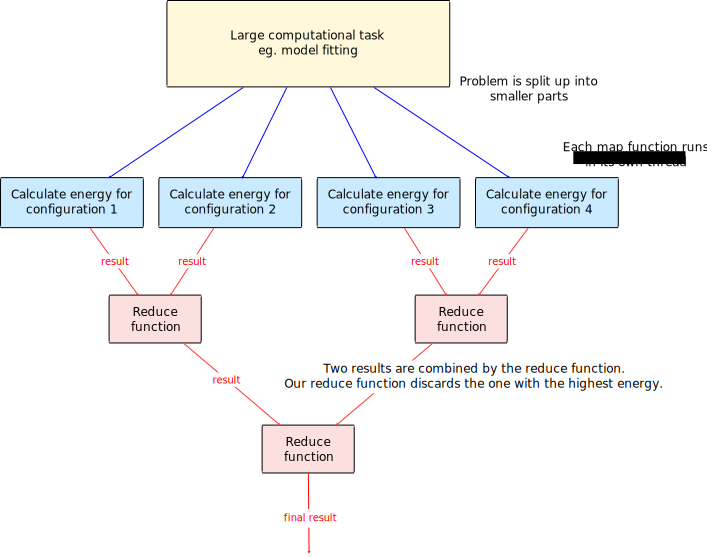
\includegraphics[width=\textwidth]{mapreduce.png}
	\caption{A diagram showing how MapReduce may be used to parallelize and speed up modelfitting.}
	\label{MapReduceDiagram}
\end{figure}

\subsection{Lookup caching}

The most expensive functions in the modelfitting algorithm shown in Listing \ref{leastsquarescode} are those which search for nearby voxels of a given type.
These lookups are repeated over and over again as the algorithm ``moves'' the mesh around the voxel-space.
In fact, with a 41x41x11x11 parameter space and 319 points in the mesh, almost 65 million ``how far is the nearest voxel'' queries are performed.
In the worst case, where the mesh is nowhere near the actual limb it is searching for, this could lead to a total of 86,361 million calls to the Voxel\_Space's get() function.

Clearly the result of these requests will always be the same for any given input.
The closest edge voxel to some arbitrary point in the space is not going to change depending on the model parameters, so recalculating it every time is unnecessary.
Caching the results of these lookups could improve algorithm execution time dramatically.

A 44MB cache is allocated and initalised at the start of the algorithm's execution.
This cache is big enough to hold two 4-byte floats for every voxel in the space.
The first float is used to store the distance from that voxel to any other filled voxel, and the second float is used to store the distance to an edge voxel.
As the algorithm runs, the distanceToEdgeVoxel and distanceToVoxel functions add their results to the proper place in the cache.
Future calls to these functions can then reuse the previously computed values.

The only down-side to this approach is that collisions can occur when two threads try to perform the same lookup at the same time.
Both threads will query the cache at the same location and see that no value has been written yet, so they will both begin to calculate the same value.
The first thread to finish will write the result to the cache, and the second thread will overwrite it with exactly the same value.
This situation is depicted in Figure \ref{CacheCollisions}.

\begin{figure}[tb]
	\centering
	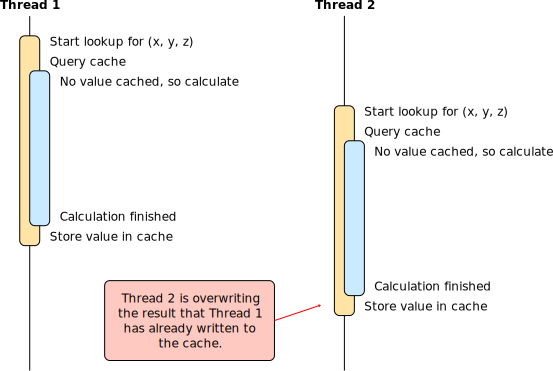
\includegraphics[width=\textwidth]{cachecollisions.png}
	\caption{Multiple threads can waste time computing identical values.}
	\label{CacheCollisions}
\end{figure}

No unwanted behaviour actually results from this situation - the worst that happens is that a little bit of time is wasted and the second thread overwrites the first thread's result with an identical value.
Writing to the cache is an atomic operation so there is no need to wrap cache access in costly mutex locking and unlocking.
As can be seen in Table \ref{CacheStatsTable}, the number of cache collisions is relatively small compared to the number of successful cache hits and cache misses, although obviously the number will increase as more processor cores are added.

\begin{table}[thb]
	\centering
	\begin{tabular}{|l|c|c|}
		\hline
		Cache hits & 67,000,000 \\
		Cache misses & 1,000,000 \\
		Cache collisions & 4,000 \\
		\hline
	\end{tabular}
	\caption{Cache statistics generated by fitting to Frame 81 of Sample 81.
		Each cache hit represents time saved by not having to search the voxel space.}
	\label{CacheStatsTable}
\end{table}

Implementing this cache reduced execution time of Sample 81 Frame 81 from 2 hours to 1 minute 45 seconds.

\subsection{Multi-resolution search}
\label{Design:MultiRes}

\begin{figure}[tb]
	\centering
	\subfloat[First pass]{\label{MultiResImage1}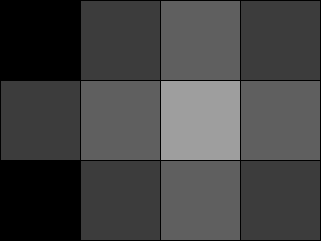
\includegraphics[width=5cm]{multires1.png}}
	\qquad
	\subfloat[Second pass]{\label{MultiResImage2}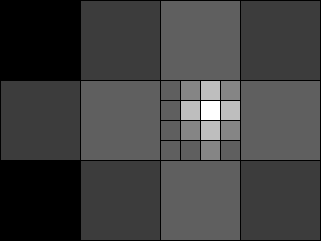
\includegraphics[width=5cm]{multires2.png}}
	\caption{The multiresolution search approach uses two passes - the first is at a low resolution over a large area,
		and the second is at a high resolution over a small area.}
	\label{MultiResImages}
\end{figure}

Our initial algorithm in Listing \ref{leastsquarescode} searches over the whole parameter space at a fixed resolution (41 samples for $\theta$ and 11 samples for $\alpha$).
Because the parameter space is four-dimensional, this leads to the algorithm evaluating the energy function $41*41*11*11 = 203401$ times.

We can improve on this by noticing that in the vast majority of the energy plots there is only one minimum.
If we run one search over the whole parameter space at a low resolution, we can then run a second high resolution search centered on the minimum found by the first search.
This will save us sampling the energy function in thousands of places where there can't possibly be a minimum.
Figure \ref{MultiResImages} demonstrates the principle behind this idea - the second pass is centered on the minimum found in the first pass.

The visualisation presented in Figure \ref{MultiResImages} is perhaps slightly misleading.
The large shaded areas do not represent an average of many samples within their bounds, but rather the result of a single sample in their centre.
It is important to consider the size of area around a first-pass minimum that would need to be sampled at a higher resolution to ensure we find the correct result.

We can define this error as such:

\begin{align}
	E_\theta &= 2 * \frac{\text{range}_\theta}{\text{resolution}_\theta - 1} \\
	E_\alpha &= 2 * \frac{\text{range}_\alpha}{\text{resolution}_\alpha - 1}
\end{align}

This means that the dimensions of the area to be searched at high resolution are twice the distance between samples at the lower resolution.

One concern about multi-resolution search is with the assumption that there is only one minimum in the parameter space.
The low resolution samples in the first pass may fall either side of the global minimum but have higher energies than one that falls right on another local minimum.
This would lead to the second pass centering its search around the local minimum and missing the true solution.
While this is a valid concern, in practice it was found to make very little difference to the results when tested over a large series of frames.

\subsection{Quantifying the improvements}

\begin{table}[thb]
	\centering
	\begin{tabular}{l|l}
		\hline
		Method & Execution time \\
		\hline
		High resolution search & 1 hour 55 minutes \\
		Low resolution search & 1 hour \\
		with mapreduce & 35 minutes \\
		with cache & 1 minute 45 seconds \\
		with loop optimisation & 44 seconds \\
		with multiresolution & 7 seconds \\
		\hline
	\end{tabular}
	\caption{Execution times of the modelfitting process after making each optimisation.
		Optimisations are cumulative, so each row includes the optimisations of the rows above it.
		The ``loop optimisation'' improvement was not noteworthy enough for a mention in the previous sections,
		but involves low-level optimisation of inner loop code.
		All tests were run on an Intel Core 2 Duo 2.20GHz, and the binary was compiled without GCC optimisations (\texttt{-O0}).}
	\label{QuantifyingOptimisations}
\end{table}

